\documentclass{article}

\usepackage{fancyhdr}
\usepackage{extramarks}
\usepackage{amsmath}
\usepackage{amsthm}
\usepackage{amsfonts}
\usepackage{tikz}
\usepackage[plain]{algorithm}
\usepackage{algpseudocode}
\usepackage{graphicx}
\usepackage{gensymb}
\usepackage{calc}
\usepackage[framed,numbered,autolinebreaks,useliterate]{mcode}
\usepackage{listings}
\usepackage{empheq}
\usepackage{enumitem}
\usepackage[font=footnotesize]{caption}
\usepackage{subcaption}

\graphicspath{{./images/}}

\usetikzlibrary{automata,positioning}

%
% Basic Document Settings
%

\topmargin=-0.45in
\evensidemargin=0in
\oddsidemargin=0in
\textwidth=6.5in
\textheight=9.0in
\headsep=0.25in

\linespread{1.1}

\pagestyle{fancy}
\lhead{\hmwkAuthorLastNames}
\chead{\hmwkClass\ \hmwkTitle}
\rhead{\firstxmark}
\lfoot{\lastxmark}
\cfoot{\thepage}

\renewcommand\headrulewidth{0.4pt}
\renewcommand\footrulewidth{0.4pt}

\setlength\parindent{0pt}

%
% Create Problem Sections
%

\newcommand{\enterProblemHeader}[1]{
    \nobreak\extramarks{}{Problem {#1} continued on next page\ldots}\nobreak{}
    \nobreak\extramarks{{#1} (continued)}{{#1} continued on next page\ldots}\nobreak{}
}

\newcommand{\exitProblemHeader}[1]{
    \nobreak\extramarks{{#1} (continued)}{{#1} continued on next page\ldots}\nobreak{}
    % \stepcounter{#1}
    \nobreak\extramarks{{#1}}{}\nobreak{}
}

\setcounter{secnumdepth}{0}
\newcounter{partCounter}

\newcommand{\problemNumber}{0.0}

\newenvironment{homeworkProblem}[1][-1]{
    \renewcommand{\problemNumber}{{#1}}
    \section{\problemNumber}
    \setcounter{partCounter}{1}
    \enterProblemHeader{\problemNumber}
}{
    \exitProblemHeader{\problemNumber}
}

%
% Homework Details
%   - Title
%   - Class
%   - Author
%

\newcommand{\hmwkTitle}{Group Assignment\ \#1}
\newcommand{\hmwkClass}{RBE 500}
\newcommand{\hmwkAuthorName}{\textbf{Joshua Gross, Arjan Gupta, Melissa Kelly}}
\newcommand{\hmwkAuthorLastNames}{\textbf{Gross, Gupta, Kelly}}

%
% Title Page
%

\title{
    \vspace{2in}
    \textmd{\textbf{\hmwkClass\ \hmwkTitle}}\\
    \vspace{3in}
}

\author{\hmwkAuthorName}
\date{}

\renewcommand{\part}[1]{\textbf{\large Part \Alph{partCounter}}\stepcounter{partCounter}\\}

%
% Various Helper Commands
%

% Useful for algorithms
\newcommand{\alg}[1]{\textsc{\bfseries \footnotesize #1}}

% For derivatives
\newcommand{\deriv}[2]{\frac{\mathrm{d}}{\mathrm{d}#2} \left(#1\right)}

% For compact derivatives
\newcommand{\derivcomp}[2]{\frac{\mathrm{d}#1}{\mathrm{d}#2}}

% For partial derivatives
\newcommand{\pderiv}[2]{\frac{\partial}{\partial #2} \left(#1\right)}

% For compact partial derivatives
\newcommand{\pderivcomp}[2]{\frac{\partial #1}{\partial #2}}

% Integral dx
\newcommand{\dx}{\mathrm{d}x}

% Alias for the Solution section header
\newcommand{\solution}{\textbf{\large Solution}}

% Probability commands: Expectation, Variance, Covariance, Bias
\newcommand{\E}{\mathrm{E}}
\newcommand{\Var}{\mathrm{Var}}
\newcommand{\Cov}{\mathrm{Cov}}
\newcommand{\Bias}{\mathrm{Bias}}

\newlength\dlf% Define a new measure, dlf
\newcommand\alignedbox[2]{
% Argument #1 = before & if there were no box (lhs)
% Argument #2 = after & if there were no box (rhs)
&  % Alignment sign of the line
{
\settowidth\dlf{$\displaystyle #1$}  
    % The width of \dlf is the width of the lhs, with a displaystyle font
\addtolength\dlf{\fboxsep+\fboxrule}  
    % Add to it the distance to the box, and the width of the line of the box
\hspace{-\dlf}  
    % Move everything dlf units to the left, so that & #1 #2 is aligned under #1 & #2
\boxed{#1 #2}
    % Put a box around lhs and rhs
}
}

\begin{document}

\maketitle

\nobreak\extramarks{Problem 1}{}\nobreak{}

\pagebreak

\begin{homeworkProblem}[Problem 1]
    \subsection{Create SCARA Robot in Gazebo}

    The 3 DOF SCARA robot we have built is shown below.

    \begin{figure}[h]
        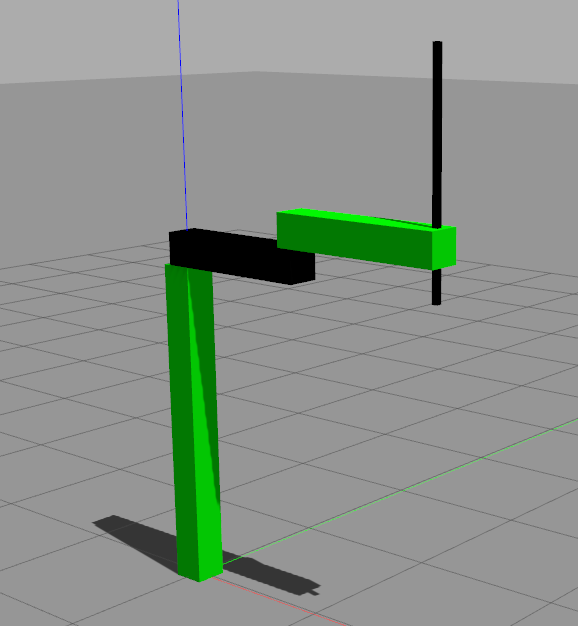
\includegraphics[scale=0.47]{gazebo-final-scara.png}
        \centering
        \caption{Final SCARA built by our team}
    \end{figure}

    We undertook the following steps to create our SCARA robot.

    \subsubsection{1 --- Modify joint locations}

    In the downloaded package, the RRBot robot has its revolute joints on the `sides' of its links, as shown in the following figure.
    
    \begin{figure}[h]
        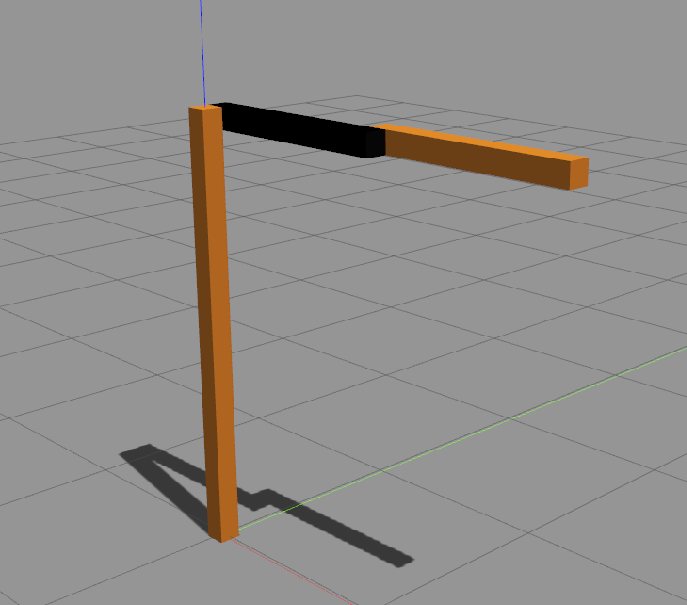
\includegraphics[scale=0.24]{initial-rrbot.png}
        \centering
        \caption{Initial RRBot in Gazebo}
    \end{figure}

    However, for a standard SCARA robot, we want the revolute joints to sweep angles in the XY plane of the world frame, not in the XZ plane.
    
    Hence, we edited the \lstinline{<joint>} element blocks in the URDF file rrbot\_description.urdf.xacro. For the first joint, we made the following
    change.

    \lstinputlisting[language=XML, firstline=51,lastline=59]{../ros2-code/src/rrbot_simulation_files/rrbot_description/urdf/rrbot_description.urdf.xacro}
    \vspace{0.15in}

    In the above code snippet, we changed the type attribute of the joint element from continuous to revolute. We also added the limit sub-element, and
    modified the origin and axis sub-elements. We made similar changes for the second joint, for which the code snippet is shown below.

    \lstinputlisting[language=XML, firstline=87,lastline=95]{../ros2-code/src/rrbot_simulation_files/rrbot_description/urdf/rrbot_description.urdf.xacro}
    \vspace{0.15in}

    As a result, our robot now looked like the following image.

    \begin{figure}[h]
        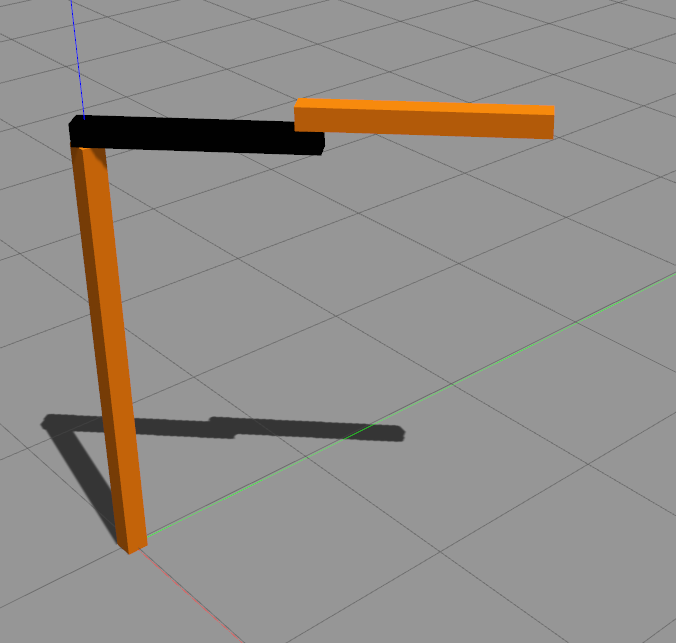
\includegraphics[scale=0.25]{top-joints-rrbot.png}
        \centering
        \caption{RRBot with top-joints}
    \end{figure}

    In order to test our changes, we moved our robot by publishing joint values in the format of the following ROS command in our terminal.\\
    \vspace{0.05in}

    \begin{lstlisting}[language=sh]
        ros2 topic pub --once /forward_position_controller/commands std_msgs/msg/Float64MultiArray "{data: [0.75 0.82]}"
    \end{lstlisting}

    \subsubsection{2 --- Add prismatic joint}

    Now our revolute joints resemble those of a SCARA robot, but we still need a prismatic joint. In order to do this, we first made the following
    changes to the rrbot\_description.urdf.xacro file.

    \lstinputlisting[language=XML, firstline=123,lastline=158]{../ros2-code/src/rrbot_simulation_files/rrbot_description/urdf/rrbot_description.urdf.xacro}
    \vspace{0.15in}

    In the above code snippet, we have changed the tool joint from fixed to prismatic, defined its translation axis, set its limits, and defined its origin.
    We defined a special \lstinline{prismatic_width} so that we could make the tool link thinner than the regular links. We also defined a
    \lstinline{prismatic_offset} so that the tool link is slightly `lowered'. This makes it so that the zero position of the tool link is at the
    same height as our first link, which makes our calculations consistent with our forward-kinematics derivation.\\

    Next, we defined the tool joint in the rrbot.ros2\_control.xacro file, so that the command and state interfaces for ROS2 could be made available 
    for that joint. Finally, we also edited the gazebo\_controllers.yaml file to define the tool joint as part of the three
    controllers --- \lstinline{forward_position_controller}, 
    \lstinline{forward_velocity_controller}, and \lstinline{forward_effort_controller}. All these modified files have been included as part of our submission
    inside the rrbot\_description.zip compressed directory.

    At this point, our robot looked as follows.
    
    \begin{figure}[h]
        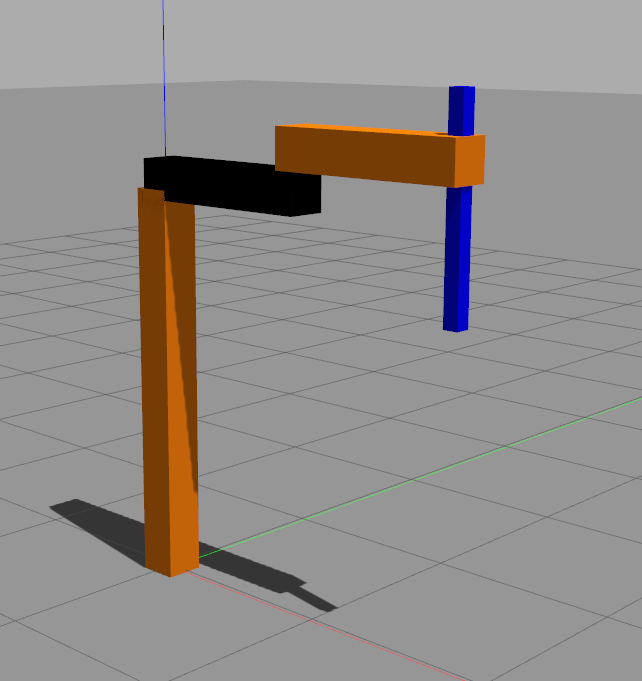
\includegraphics[scale=0.25]{unfinished-scara.png}
        \centering
        \caption{SCARA configuration without finishing touches}
    \end{figure}

    After this, we tweaked some offsets, adjusted some link lengths, changed the colors of the robot, and decreased the thickness of the tool link in order
    to arrive at our finished implementation of the SCARA robot. We also used the same ROS command as earlier (except with 3 data-points this time) to ensure
    that we were able to move all the joints of our robot.

\end{homeworkProblem}

\nobreak\extramarks{Question 2}{}\nobreak{}

\begin{homeworkProblem}[Question 2]
    \subsection{Forward Kinematics for SCARA}

    Before implementing forward kinematics in ROS, we worked out a derivation for the forward kinematics of the SCARA robot model.

    \subsubsection{Derviation}

    The image below shows the frame assignments for the robot.
    
    \begin{figure}[h]
        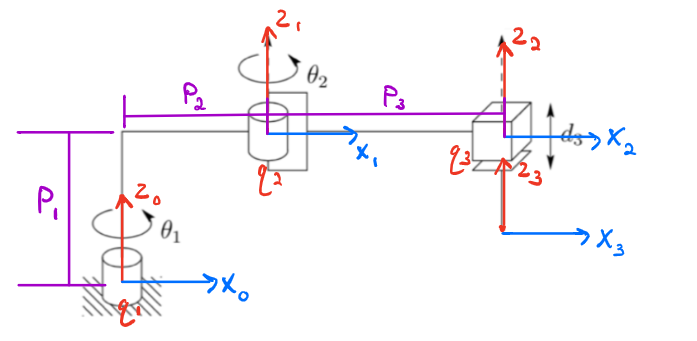
\includegraphics[scale=0.4]{fwd-kin-frames-whitebg.png}
        \centering
        \caption{Frame assignments for forward kinematics}
    \end{figure}

    Based on this, we can form the DH table as shown below.
    
    \begin{table}[h!]
        \begin{center}
            \begin{tabular}{|c|c|c|c|c|}
            \hline
            Link & $\alpha_i$ & $a_i$ & $\theta_i$ & $d_i$ \\
            \hline
            1 & 0 & $p_2$ & $q_1$ & $p_1$ \\
            2 & 0 & $p_3$ & $q_2$ & 0\\
            3 & 0 & 0 & 0 & $q_3$ \\
            \hline
            \end{tabular}
        \end{center}
    \end{table}

    Next, we create a MATLAB script as shown below. We use the matrix obtained from equation 3.10 of the textbook to write \(A_1, A_2, A_3\). By multiplying 
    these matrices, we obtain the $T^0_3$.

    \lstinputlisting[language=MATLAB]{Project_Part1_fk.m}

    \vspace{0.25in}

    This MATLAB script gives us the following $T^0_3$ matrix, which is the homogeneous transformation for the end-effector with respect to the base frame. 

    \[
        \begin{bmatrix}\cos{q_1}\,\cos{q_2}-\sin{q_1}\,\sin{q_2} & -\cos{q_1}\,\sin{q_2}-\cos{q_2}\,\sin{q_1} & 0 & P_{2}\,\cos{q_1}+P_{3}\,\cos{q_1}\,\cos{q_2}-P_{3}\,\sin{q_1}\,\sin{q_2}\\ \cos{q_1}\,\sin{q_2}+\cos{q_2}\,\sin{q_1} & \cos{q_1}\,\cos{q_2}-\sin{q_1}\,\sin{q_2} & 0 & P_{2}\,\sin{q_1}+P_{3}\,\cos{q_1}\,\sin{q_2}+P_{3}\,\cos{q_2}\,\sin{q_1}\\ 0 & 0 & 1 & P_{1}+q_{3}\\ 0 & 0 & 0 & 1 \end{bmatrix}
    \]

    \vspace{0.5in}

    \subsubsection{ROS Implementation of Forward Kinematics}

    \vspace{0.15in}

    For implementing the forward kinematics in ROS, a new package was created (this package has been submitted as a zip file along with this report).
    Inside this package, a file was created to house all of the code for the forward kinematics subscriber, calculations, and 
    publisher. In the code, we first create the Subscriber class which houses both the 
    \lstinline{__init__} and \lstinline{calculate_forward_kinematics} functions. The \lstinline{__init__} function initializes certain attributes 
    to be used later. Here, the link lengths, as provided by the Gazebo model, are defined. Next, the 
    subscriber and publisher are each created and defined by their respective message types and topics. 
    Inside of the \lstinline{calculate_forward_kinematics} function, the message containing each joint value is 
    accepted and split apart into each individual value as a variable. These joint values, along with the link 
    lengths are then plugged into the overall transformation matrix as previously calculated by hand and 
    solved with Matlab. From this 3x4 matrix, the first three rows and columns are extracted as the rotation 
    matrix. Once this matrix is obtained, an open source scipy package is used to calculate the quaternion. 
    Elements of the rotation matrix as well as the quaternion are then extracted and placed into the pose, 
    which will be published. Once this pose message is published, it can be accessed through terminal to 
    obtain the location of the end effector. Below are the commands used with this system to obtain the 
    desired results: 
    \begin{lstlisting}[language=sh]
        # Moves the Gazebo robot to the desired position
        ros2 topic pub --once /forward_position_controller/commands std_msgs/msg/Float64MultiArray "{data: [0.349066 0.610865 0.5]}"
        # Kicks off the subscriber so that it can start calculating from the joint values that are repeatedly published
        ros2 run group_project calculate
    \end{lstlisting}
    
    \vspace{0.5in}
    \subsubsection{Gazebo Screenshots with ROS Output}
    \vspace{0.15in}

    \underline{Pose 1}

    First we moved our SCARA robot by changing the joint values to $q_1 = 20\degree$, $q_2 = 35\degree$, $q_3 = 0.5$. We did this by executing the
    following command
    \begin{lstlisting}[language=sh]
        ros2 topic pub --once /forward_position_controller/commands std_msgs/msg/Float64MultiArray "{data: [0.349066 0.610865 0.5]}"
    \end{lstlisting}

    Next, we launced our forward kinematics calculation ROS node. The screenshots obtained are shown in Figure 6.

    \begin{figure}[h]
        \begin{subfigure}[b]{0.5\textwidth}
            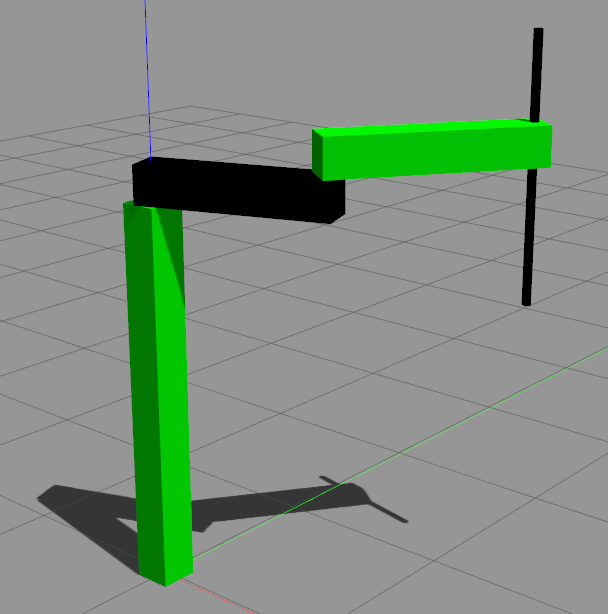
\includegraphics[scale=0.35]{fwd-kin-pose1.png}
            \centering
            \caption{Gazebo robot screenshot}
        \end{subfigure}
        \begin{subfigure}[b]{0.5\textwidth}
            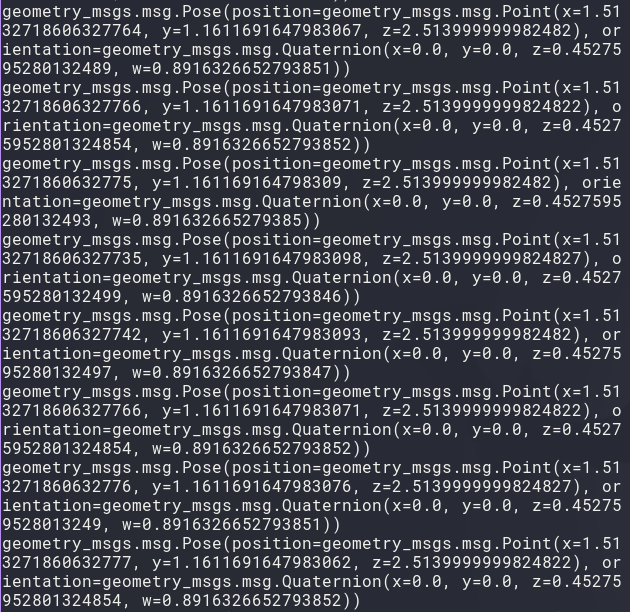
\includegraphics[scale=0.35]{fwd-kin-termoutput1.png}
            \centering
            \caption{Terminal output screenshot}
        \end{subfigure}
        \caption{Pose 1 Screenshots}
    \end{figure}


    \vspace{1in}

    \underline{Pose 2}

    We moved our SCARA robot by setting the joint values to $q_1 = 72\degree$, $q_2 = 28\degree$, $q_3 = 1.05$. We did this by executing the following command

    \begin{lstlisting}[language=sh]
        ros2 topic pub --once /forward_position_controller/commands std_msgs/msg/Float64MultiArray "{data: [1.25664 0.488692 1.05]}"
    \end{lstlisting}

    After this we launched the forward kinematics ROS node as well. The obtained screenshots are shown in Figure 7.

    \begin{figure}[h]
        \begin{subfigure}[b]{0.5\textwidth}
            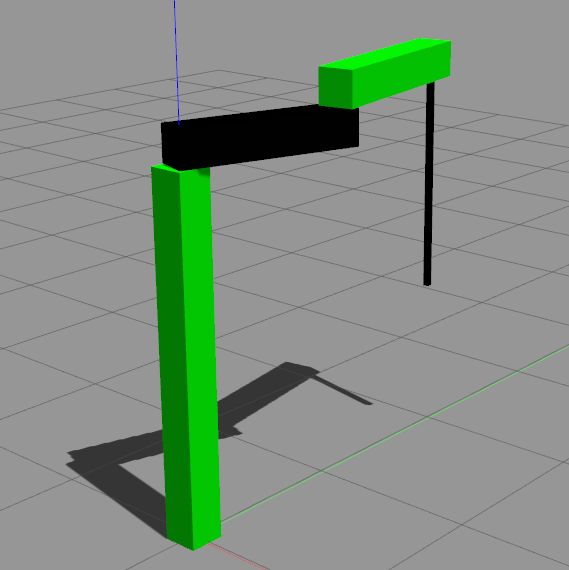
\includegraphics[scale=0.35]{fwd-kin-pose2.png}
            \centering
            \caption{Gazebo robot screenshot}
        \end{subfigure}
        \begin{subfigure}[b]{0.5\textwidth}
            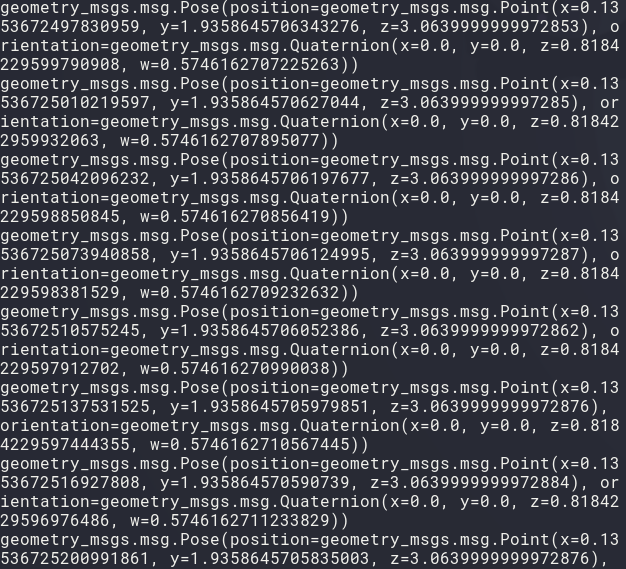
\includegraphics[scale=0.35]{fwd-kin-termoutput2.png}
            \centering
            \caption{Terminal output screenshot}
        \end{subfigure}
        \caption{Pose 2 Screenshots}
    \end{figure}

    \underline{Pose 3}

    \begin{figure}[h]
        \begin{subfigure}[b]{0.5\textwidth}
            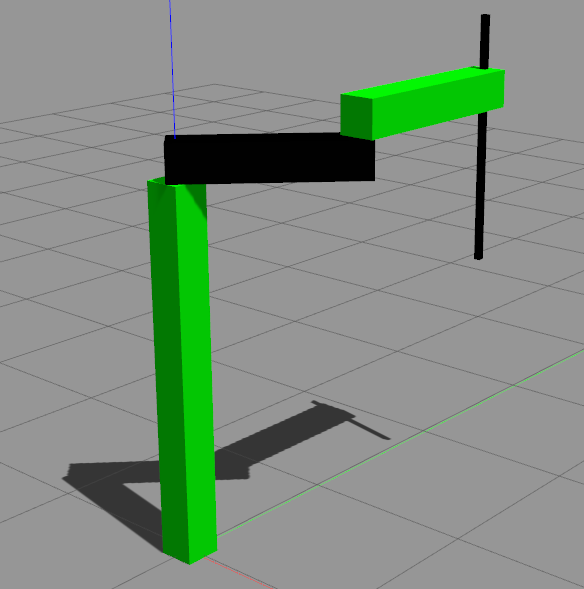
\includegraphics[scale=0.35]{fwd-kin-pose3.png}
            \centering
            \caption{Gazebo robot screenshot}
        \end{subfigure}
        \begin{subfigure}[b]{0.5\textwidth}
            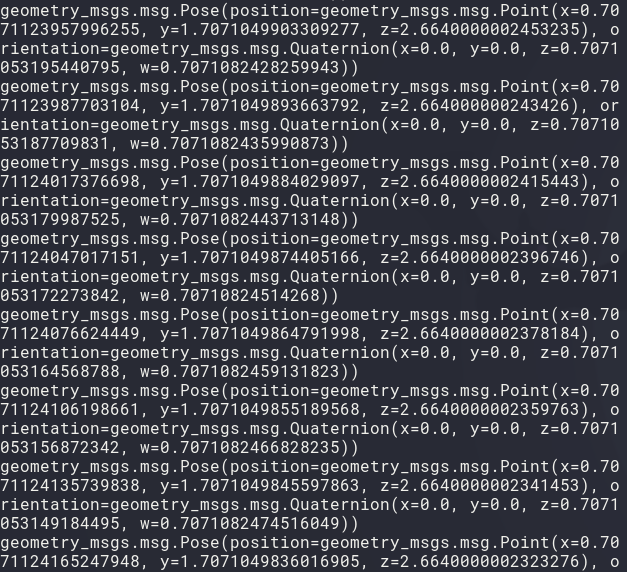
\includegraphics[scale=0.35]{fwd-kin-termoutput3.png}
            \centering
            \caption{Terminal output screenshot}
        \end{subfigure}
        \caption{Pose 3 Screenshots}
    \end{figure}

    We moved our SCARA robot by setting the joint values to $q_1 = 45\degree$, $q_2 = 45\degree$, $q_3 = 0.65$. We did this by executing the following command

    \begin{lstlisting}[language=sh]
        ros2 topic pub --once /forward_position_controller/commands std_msgs/msg/Float64MultiArray "{data: [0.785398 0.785398 0.65]}"
    \end{lstlisting}

    After this we launched the forward kinematics ROS node as well. The obtained screenshots are shown in Figure 8


\end{homeworkProblem}

\nobreak\extramarks{Question 3}{}\nobreak{}

\begin{homeworkProblem}[Question 3]
    \subsection{Inverse Kinematics for SCARA}
    Before implementing forward kinematics in ROS, we worked out a derivation for the inverse kinematics of the SCARA robot model.
    
    \subsubsection{Derviation}

    For the inverse kinematics, a side view and a top view were used to geometrically solve for the unknown joint values.\\
    \vspace{0.05in}\\
    \underline{Top view}
    \vspace{0.1in}
    \begin{figure}[h]
        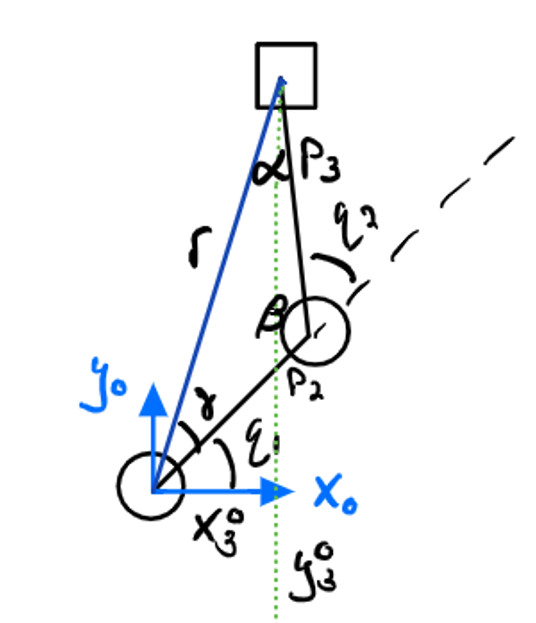
\includegraphics[scale=0.55]{top-view-inv-kin.png}
        \centering
        \caption{Top view for inverse kinematics}
    \end{figure}
    
    From Figure 9, $q_1$ can be expressed as
    \begin{align*}
        \boxed{q_1 = \arctan \left( \frac{y^0_3}{x^0_3} \right) - \gamma}
    \end{align*}
    Similarly, $q_2$ can be expressed as,
    \begin{align*}
        \alignedbox{q_2}{= 180\degree - \beta}
    \end{align*}

    In order to find $\alpha$ and $\gamma$, we can use the law of cosines. For instance, $\alpha$ can be found as follows,
    \begin{align*}
        &{P_2}^2 = r^2 + {P_3}^2 - 2 r P_3 \cos \alpha\\
        &2 r P_3 \cos \alpha = r^2 + {P_3}^2 - {P_2}^2\\
        &\alpha = \arccos \left( \frac{r^2 + {P_3}^2 - {P_2}^2}{2 r P_3} \right)
    \end{align*}

    Similarly, $\gamma$ can be expressed as,

    \[
        \gamma = \arccos \left( \frac{r^2 + {P_2}^2 - {P_3}^2}{2 r P_3} \right)
    \]

    Hence, $\beta$ can be written as,
    \[
        \beta = 180\degree - \alpha - \gamma
    \]

    Also, we can express r in its norm,
    \[
        r = \sqrt{{(y^0_3)}^2 + {(x^0_3)}^2}
    \]

    \underline{Side view}
    \begin{figure}[h]
        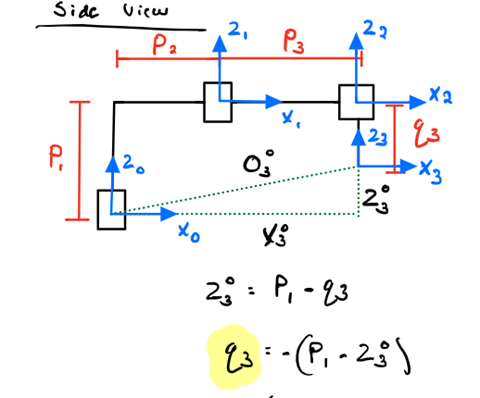
\includegraphics[scale=0.47]{side-view-inv-kin.png}
        \centering
        \caption{Side view for inverse kinematics}
    \end{figure}

    From Figure 10, we can find $q_3$ as follows
    \begin{align*}
        z^0_3 &= P_1 - q_3\\
        \alignedbox{q_3}{= -(P_1 - z^0_3)}
    \end{align*}\\

    Now we have expressed all the joint variables in the form of constants of the system and end-effector position coordinates.
    These equations for each joint value can now be solved once the end effector location is known.\\
    In the following MATLAB script, these equations are written out, and when plugging in the 
    values found in the forward kinematics, the original joint values are found, therefore 
    proving their accuracy.

    \lstinputlisting{Project_Part1_full.m}
    \vspace{0.1in}
    Both the forward and inverse kinematics are now solved and ready to be plugged into ROS.

    \vspace{0.3in}
    \subsubsection{ROS Implementation of Inverse Kinematics}
    \vspace{0.1in}

    For implementing the ROS portion of inverse kinematics, we need to implement a service. However,
    before implementing the service itself we need a custom interface for the request/response structure
    of the service. Hence, we created a new CMake package called \lstinline{rbe_custom_interfaces}.
    Under this package, we created a new directory srv, in which we defined our custom
    \lstinline{InvKinSCARA.srv} file. After this, we edited the CMakeLists to import the
    \lstinline{rosidl_default_generators} so that our custom interface could be generated
    in the intended manner in ROS.\@ Our custom interface is then built and loaded locally
    using \lstinline{. install/setup.bash}.\\
    \vspace{0.02in}\\
    After our custom interface became ready, we created a new ROS Python package called
    \lstinline{inv_kin_serv}.\\ Inside this package, under the directory of the same name as the package,
    we created a file called\\ \lstinline{inverse_kin_service.py}. Inside this file, we declared
    a class for our service, which we called \lstinline{InverseKinService}. The constructor of this
    class initializes its super class and assigns the link-lengths of our robot system as its member
    variables. The constructor then creates our service, which uses our custom interface, and
    assigns a callback function called \lstinline{calculate_inverse_kin} that we have defined.
    This \lstinline{calculate_inverse_kin} function calculates the joint variables from the end-effector
    position, as we have shown in the preceding Derviation section. After building our package, we used
    the following commands run and communicate with it.

    \begin{lstlisting}[language=sh]
        # This command launches our service, which waits for a "call", or client request.
        ros2 run inv_kin_serv service
        # This command calls out to the service
        ros2 service call /inverse_kin_service rbe500_custom_interfaces/srv/InvKinSCARA "{x: 1.5133, y: 1.1612, z: 2.5}"
    \end{lstlisting}

    \vspace{0.1in}

    Both ROS packages for inverse kinematics have been zipped and included in the submission with this report.

    \vspace{0.3in}
    \subsubsection{Terminal Screenshot of ROS Output}
    \vspace{0.1in}

    In the screenshot below (which has also been included in the inverse kinematics server package), we can see the calculated
    ROS output for the three end-effector positions that we used as examples in the forward kinematics portion of this report.
    Therefore this additionally proves our forward and inverse kinematics implementations.

    \begin{figure}[h]
        \centering
        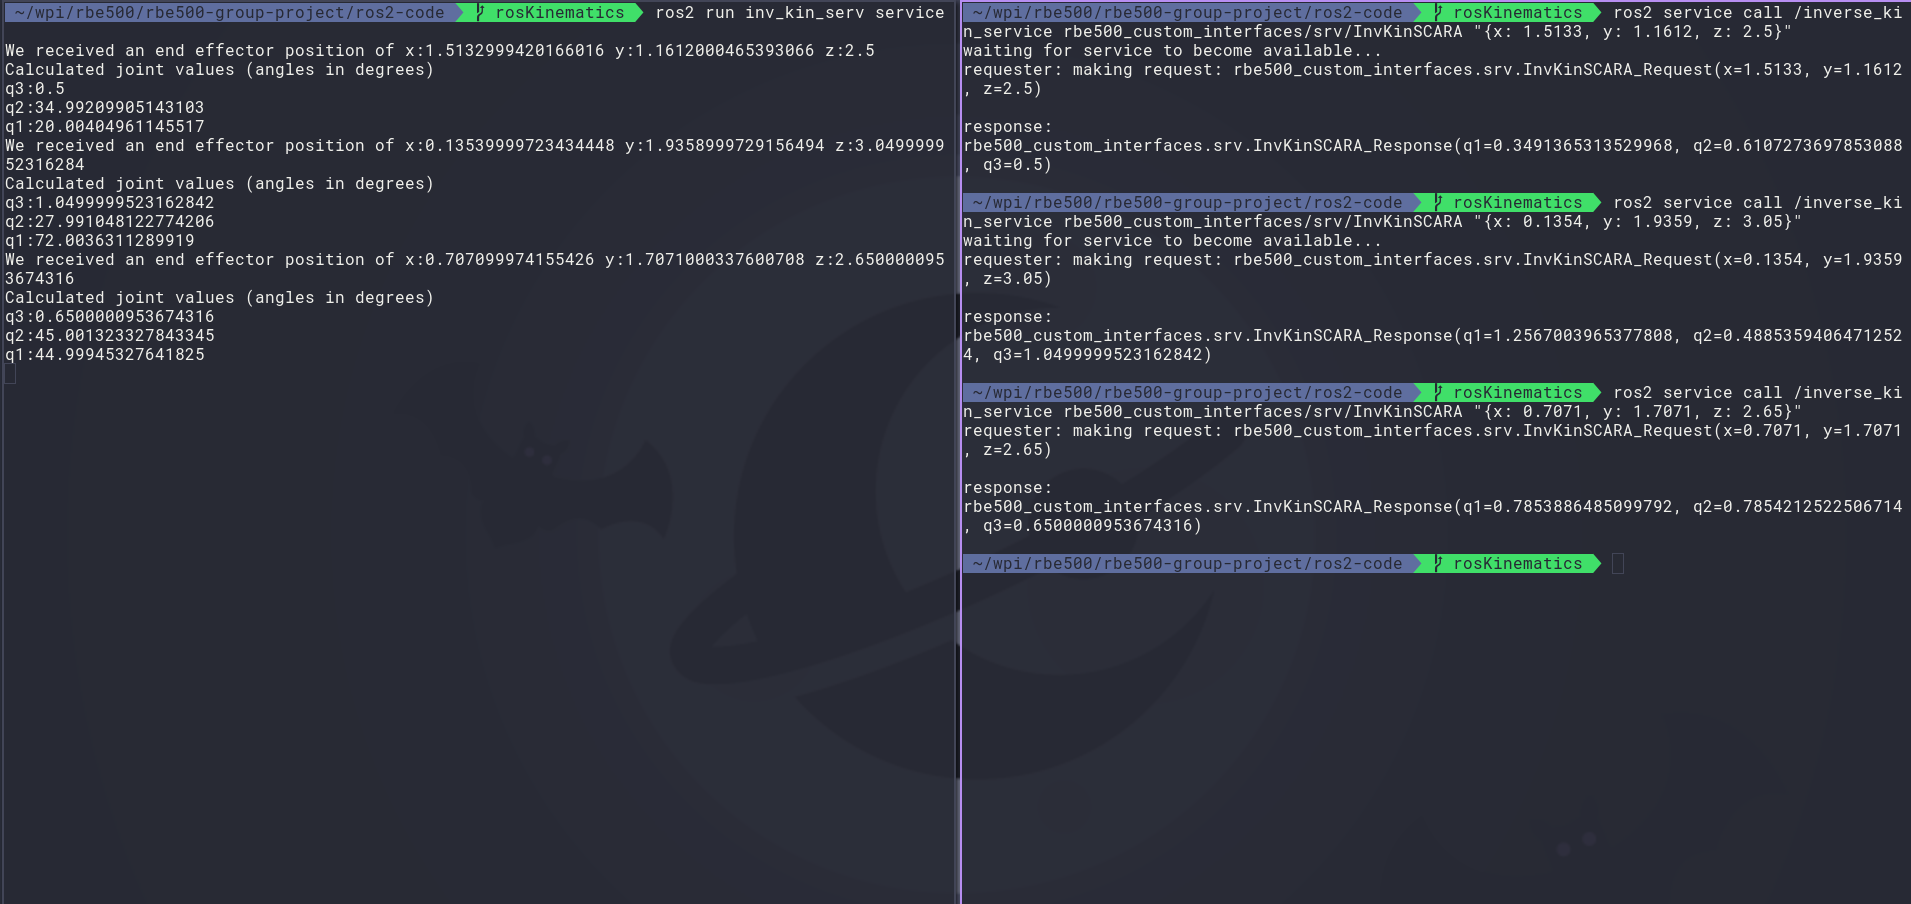
\includegraphics[width=6.5in]{inv-kin-ros-output.png}
    \end{figure}

\end{homeworkProblem}

\end{document}